% =========================================================================== %
% TeX input file: "Run the hello world application"
%
% WARNING: this tex file does not compile standalone, it needs to be embedded
% in a master tex document (e.g. Introduction.tex)
% =========================================================================== %

After the initial project creation step we can start the Scout application for the first time.
For this, we switch to the Scout Explorer view and select the root node \java{org.eclipse.scout.helloworld}.
This then loads the corresponding controls and the \textit{Product Launchers section} into the \textit{Scout Object Properties} view as shown in \figref{sdk_initial_helloworld_project}.

\begin{figure}
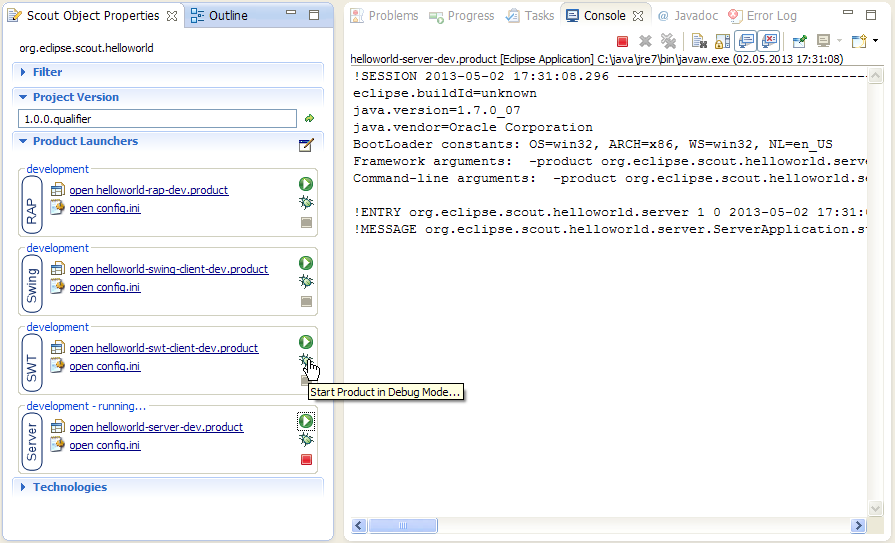
\includegraphics[width=15cm]{sdk_start_client_product.png} 
\caption{Starting the Hello World application in the Scout SDK using the provided product launcher. Make sure to start the server before starting any client product.}
\figlabel{start_client}
\index{Product launchers}
\end{figure}

In the product launcher section of the Scout Object Properties view four launcher boxes are available. 
One launcher box for the Scout server product, and three launchers for the different client products.
Each launcher box provides a link to the corresponding configuration and product definition files, as well as the launcher icons to start and stop the corresponding product.
The green \icon{Circle} starts the product in normal mode.
The \icon{Bug} just below, starts a product in debug mode.
To terminate a running product, the red \icon{Square} is provided. 

Before any of the client products is started, we need to start the server product using the green circle or the bug launcher icon.
During startup of the Scout server you should see console output similar to the one shown on the right hand side of \figref{start_client}.


Once the server is running, you may start the web client as shown in \figref{start_client}.
To start the Swing client, or the SWT client use the corresponding green \icon{Circle} or \icon{Bug}.
And with a running RAP client, the Scout web client is opened in a web browser by clicking on the provided \link{Automatic Device Dispatch}.

\begin{figure}
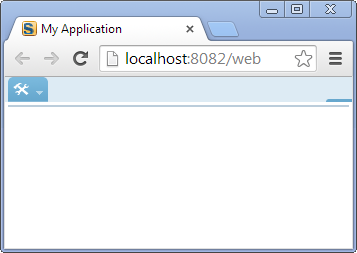
\includegraphics[width=4.5cm]{hellworld_empty_rap.png} \hspace{3mm}
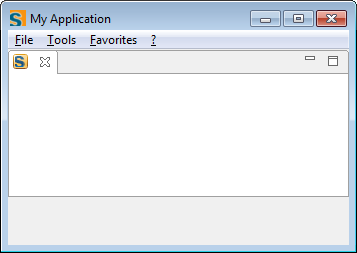
\includegraphics[width=4.5cm]{hellworld_empty_swing.png} \hspace{3mm}
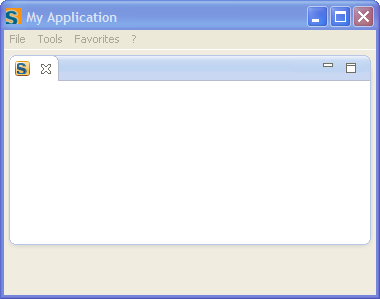
\includegraphics[width=4.5cm]{hellworld_empty_swt.png}
\caption{Running the three client applications. 
Each client displays an empty desktop form. 
The web client, the Swing client, and the SWT client}
\figlabel{helloworld_empty}
\end{figure}

Having started the Scout server and all client products, the running client applications should look as shown in \figref{helloworld_empty}.

% =========================================================================== %
% EOF TeX input file
% =========================================================================== %
